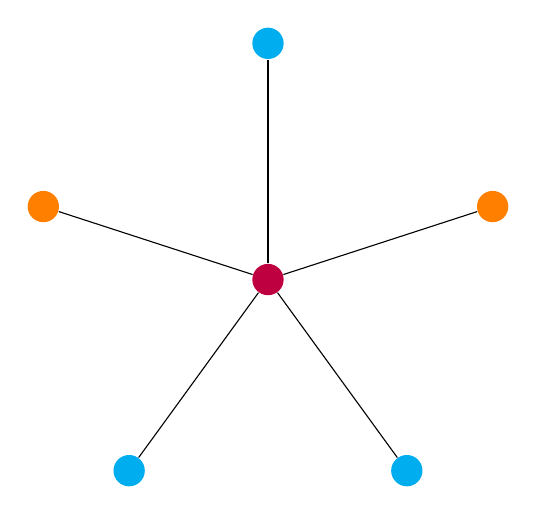
\begin{tikzpicture}[scale=2]
	
	% ---- Adjustable colors ----
	\def\centerColor{purple}
	\def\colorA{cyan}
	\def\colorB{orange}
	\def\colorC{cyan}
	\def\colorD{cyan}
	\def\colorE{orange}
	
	% ---- Positions of outer vertices (5 around a circle) ----
	\foreach \i/\name/\col in {
		90/A/\colorA,
		18/B/\colorB,
		-54/C/\colorC,
		-126/D/\colorD,
		162/E/\colorE
	}
	{
		\node[fill=\col, circle, inner sep=4pt] (v\name) at (\i:1.5) {};
	}
	
	% ---- Center vertex ----
	\node[fill=\centerColor, circle, inner sep=4pt] (center) at (0,0) {};
	
	% ---- Edges to center ----
	\foreach \name in {A,B,C,D,E}
	\draw (center) -- (v\name);
	
\end{tikzpicture}
